\chapter{Aplicas funciones trigonométricas}

\section{Funciones trigonométricas en el plano cartesiano}

Aquí están valores típicos del seno, coseno y tangente (ejercicio 2 del capítulo
VI).

  \begin{center}
  \begin{tabular}{| l | c | c | c | c | c | c | c | c | c | c | c | c | c | c | c | c |}
    \hline
    $\alpha$ &
    $-\frac{5\pi}{6}$ &
    $-\frac{3\pi}{4}$ &
    $-\frac{2\pi}{3}$ &
    $-\frac{\pi}{2}$ &
    $-\frac{\pi}{3}$ &
    $-\frac{\pi}{4}$ &
    $-\frac{\pi}{6}$ &
    $0$ &
    $\frac{\pi}{6}$ &
    $\frac{\pi}{4}$ &
    $\frac{\pi}{3}$ &
    $\frac{\pi}{2}$ &
    $\frac{2\pi}{3}$ &
    $\frac{3\pi}{4}$ &
    $\frac{5\pi}{6}$ &
    $\pi$ \\
    \hline
    $\sin \alpha$ & 
    $-\frac{1}{2}$ &
    $-\frac{\sqrt{2}}{2}$ &
    $-\frac{\sqrt{3}}{2}$ &
    $-1$ &
    $-\frac{\sqrt{3}}{2}$ &
    $-\frac{\sqrt{2}}{2}$ &
    $-\frac{1}{2}$ &
    $0$ &
    $\frac{1}{2}$ &
    $\frac{\sqrt{2}}{2}$ &
    $\frac{\sqrt{3}}{2}$ &
    $1$ &
    $\frac{\sqrt{3}}{2}$ &
    $\frac{\sqrt{2}}{2}$ &
    $\frac{1}{2}$ &
    $0$
    \\
    \hline
    $\cos \alpha$ &
    $-\frac{\sqrt{3}}{2}$ &
    $-\frac{\sqrt{2}}{2}$ &
    $-\frac{1}{2}$ &
    $0$ &
    $\frac{1}{2}$ &
    $\frac{\sqrt{2}}{2}$ &
    $\frac{\sqrt{3}}{2}$ &
    $1$ &
    $\frac{\sqrt{3}}{2}$ &
    $\frac{\sqrt{2}}{2}$ &
    $\frac{1}{2}$ &
    $0$ &
    $-\frac{1}{2}$ &
    $-\frac{\sqrt{2}}{2}$ &
    $-\frac{\sqrt{3}}{2}$ &
    $-1$
    \\
    \hline
    $\tan \alpha$ & 
    $\frac{\sqrt{3}}{3}$ &
    $1$ &
    $\sqrt{3}$ &
    / &
    $-\sqrt{3}$ &
    $-1$ &
    $-\frac{\sqrt{3}}{3}$ &
    $0$ &
    $\frac{\sqrt{3}}{3}$ &
    $1$ &
    $\sqrt{3}$ &
    / &
    $-\sqrt{3}$ &
    $-1$ &
    $-\frac{\sqrt{3}}{3}$ &
    $0$
    \\
    \hline
  \end{tabular}
  \end{center}

y sus representación gráficas en el plano cartesiano. Por que
$\sin\left(\alpha+2\pi\right) = \sin\left(\alpha\right)$,
$\cos\left(\alpha+2\pi\right) = \cos\left(\alpha\right)$ y
$\tan\left(\alpha+\pi\right)$ (ejercicio 3 del capítulo VI), las funciones son
periódicas: podemos considerar la curba sobre $[-\pi,\pi]$ (para el seno
y coseno) o sobre $]-\frac{\pi}{2}, \frac{\pi}{2}[$ (para la tangente) y
repetar esa forma para obtener las gráficas completas.

\begin{center}
  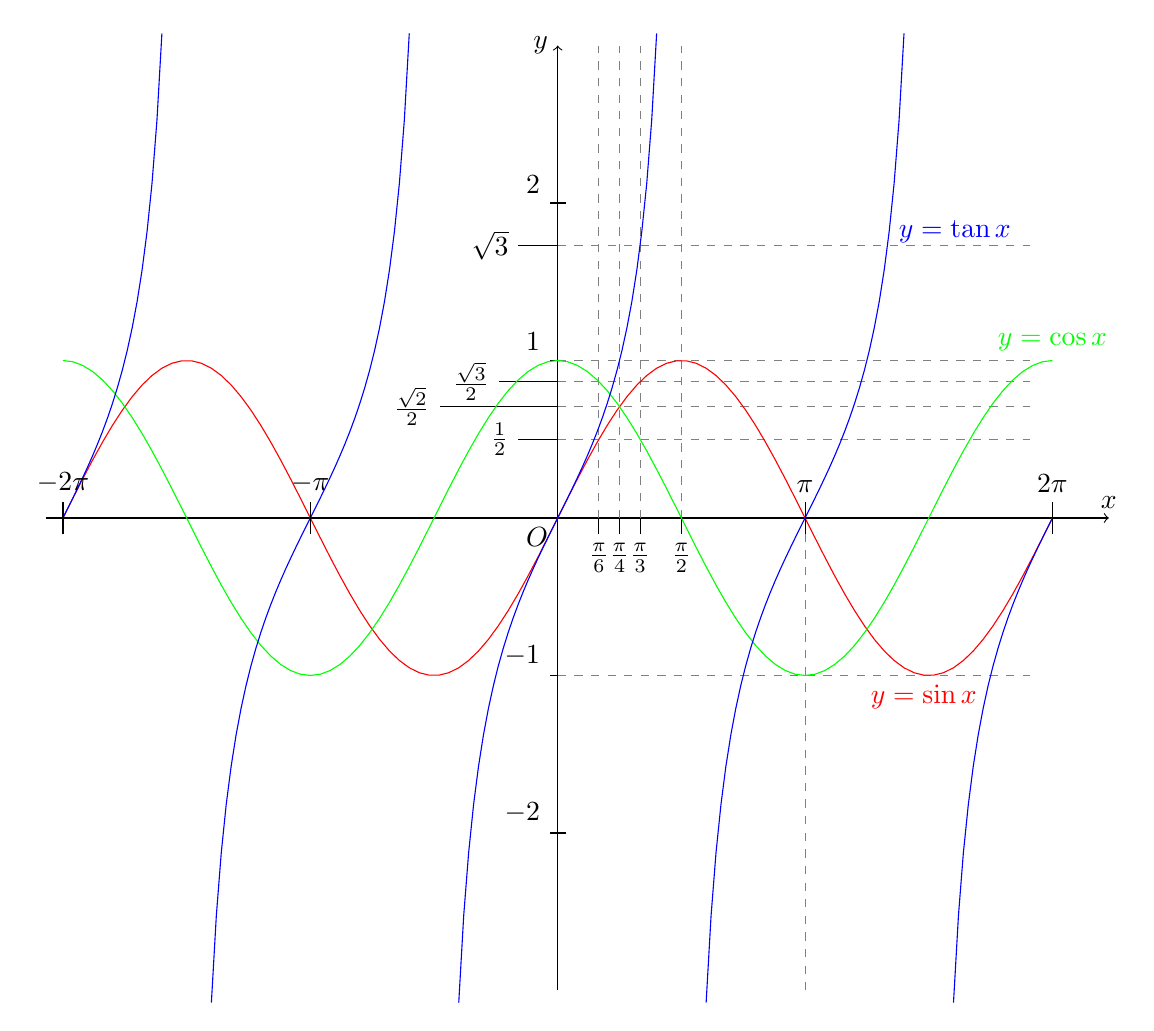
\begin{tikzpicture}[yscale=2]
    \begin{scope}
      \draw[->] (-6.5,0) -- (7,0) node[above] {$x$};
      \draw[->] (0,-3) -- (0,3) node[left] {$y$};;

      \draw[color=gray,style=dashed]
      (0.5235987755982988,0)--(0.5235987755982988,3);
      \draw(0.5235987755982988,0)--
      (0.5235987755982988,-.1) node[below]{$\frac{\pi}{6}$};
      \draw[color=gray,style=dashed]
      (0.7853981633974483,0)--(0.7853981633974483,3);
      \draw(0.7853981633974483,0)--
      (0.7853981633974483,-.1) node[below]{$\frac{\pi}{4}$};
      \draw[color=gray,style=dashed]
      (1.047197551196597,0)--(1.047197551196597,3);
      \draw(1.047197551196597,0)--
      (1.047197551196597,-.1) node[below]{$\frac{\pi}{3}$};
      \draw[color=gray,style=dashed]
      (1.570796326794896,0)--(1.570796326794896,3);
      \draw(1.570796326794896,0)--
      (1.570796326794896,-.1) node[below]{$\frac{\pi}{2}$};
      \draw[color=gray,style=dashed]
      (3.141592653589793,-3)--(3.141592653589793,0);

      \foreach \y in {-2,-1,1,2} {
        \draw(.1,\y) -- (-.1,\y) node[above left]{$\y$};
      }
      \draw[color=gray,style=dashed] (0,1)--(6,1) (0,-1) -- (6,-1);
      \draw[color=gray,style=dashed]
      (0,1.732050807568877)--(6,1.732050807568877);
      \draw(0,1.732050807568877)--(-.5,1.732050807568877)
      node[left]{$\sqrt{3}$};
      \draw[color=gray,style=dashed]
      (0,.5)--(6,.5);
      \draw(0,.5)--(-.5,.5) node[left]{$\frac{1}{2}$};

      \draw[color=gray,style=dashed]
      (0,0.8660254037844386)--(6,0.8660254037844386);
      \draw(0,0.8660254037844386)--(-.75,0.8660254037844386)
      node[left]{$\frac{\sqrt{3}}{2}$};


      \draw[color=gray,style=dashed]
      (0,0.7071067811865475)--(6,0.7071067811865475);
      \draw(0,0.7071067811865475)--(-1.5,0.7071067811865475)
      node[left]{$\frac{\sqrt{2}}{2}$};

      \draw[color=red] (-6.2832,0)--(-6.1575,0.1253)--(-6.0319,0.2487)--(-5.9062,0.3681)--(-5.7805,0.4818)--(-5.6549,0.5878)--(-5.5292,0.6845)--(-5.4035,0.7705)--(-5.2779,0.8443)--(-5.1522,0.9048)--(-5.0265,0.9511)--(-4.9009,0.9823)--(-4.7752,0.998)--(-4.6496,0.998)--(-4.5239,0.9823)--(-4.3982,0.9511)--(-4.2726,0.9048)--(-4.1469,0.8443)--(-4.0212,0.7705)--(-3.8956,0.6845)--(-3.7699,0.5878)--(-3.6442,0.4818)--(-3.5186,0.3681)--(-3.3929,0.2487)--(-3.2673,0.1253)--(-3.1416,0)--(-3.0159,-0.1253)--(-2.8903,-0.2487)--(-2.7646,-0.3681)--(-2.6389,-0.4818)--(-2.5133,-0.5878)--(-2.3876,-0.6845)--(-2.2619,-0.7705)--(-2.1363,-0.8443)--(-2.0106,-0.9048)--(-1.885,-0.9511)--(-1.7593,-0.9823)--(-1.6336,-0.998)--(-1.508,-0.998)--(-1.3823,-0.9823)--(-1.2566,-0.9511)--(-1.131,-0.9048)--(-1.0053,-0.8443)--(-0.8796,-0.7705)--(-0.754,-0.6845)--(-0.6283,-0.5878)--(-0.5027,-0.4818)--(-0.377,-0.3681)--(-0.2513,-0.2487)--(-0.1257,-0.1253)--(0,0)--(0.1257,0.1253)--(0.2513,0.2487)--(0.377,0.3681)--(0.5027,0.4818)--(0.6283,0.5878)--(0.754,0.6845)--(0.8796,0.7705)--(1.0053,0.8443)--(1.131,0.9048)--(1.2566,0.9511)--(1.3823,0.9823)--(1.508,0.998)--(1.6336,0.998)--(1.7593,0.9823)--(1.885,0.9511)--(2.0106,0.9048)--(2.1363,0.8443)--(2.2619,0.7705)--(2.3876,0.6845)--(2.5133,0.5878)--(2.6389,0.4818)--(2.7646,0.3681)--(2.8903,0.2487)--(3.0159,0.1253)--(3.1416,0)--(3.2673,-0.1253)--(3.3929,-0.2487)--(3.5186,-0.3681)--(3.6442,-0.4818)--(3.7699,-0.5878)--(3.8956,-0.6845)--(4.0212,-0.7705)--(4.1469,-0.8443)--(4.2726,-0.9048)--(4.3982,-0.9511)--(4.5239,-0.9823)--(4.6496,-0.998)node[below]{$y = \sin{x}$}--(4.7752,-0.998)--(4.9009,-0.9823)--(5.0265,-0.9511)--(5.1522,-0.9048)--(5.2779,-0.8443)--(5.4035,-0.7705)--(5.5292,-0.6845)--(5.6549,-0.5878)--(5.7805,-0.4818)--(5.9062,-0.3681)--(6.0319,-0.2487)--(6.1575,-0.1253)--(6.2832,0);
      \draw[color=green] (-6.2832,1)--(-6.1575,0.9921)--(-6.0319,0.9686)--(-5.9062,0.9298)--(-5.7805,0.8763)--(-5.6549,0.809)--(-5.5292,0.729)--(-5.4035,0.6374)--(-5.2779,0.5358)--(-5.1522,0.4258)--(-5.0265,0.309)--(-4.9009,0.1874)--(-4.7752,0.0628)--(-4.6496,-0.0628)--(-4.5239,-0.1874)--(-4.3982,-0.309)--(-4.2726,-0.4258)--(-4.1469,-0.5358)--(-4.0212,-0.6374)--(-3.8956,-0.729)--(-3.7699,-0.809)--(-3.6442,-0.8763)--(-3.5186,-0.9298)--(-3.3929,-0.9686)--(-3.2673,-0.9921)--(-3.1416,-1)--(-3.0159,-0.9921)--(-2.8903,-0.9686)--(-2.7646,-0.9298)--(-2.6389,-0.8763)--(-2.5133,-0.809)--(-2.3876,-0.729)--(-2.2619,-0.6374)--(-2.1363,-0.5358)--(-2.0106,-0.4258)--(-1.885,-0.309)--(-1.7593,-0.1874)--(-1.6336,-0.0628)--(-1.508,0.0628)--(-1.3823,0.1874)--(-1.2566,0.309)--(-1.131,0.4258)--(-1.0053,0.5358)--(-0.8796,0.6374)--(-0.754,0.729)--(-0.6283,0.809)--(-0.5027,0.8763)--(-0.377,0.9298)--(-0.2513,0.9686)--(-0.1257,0.9921)--(0,1)--(0.1257,0.9921)--(0.2513,0.9686)--(0.377,0.9298)--(0.5027,0.8763)--(0.6283,0.809)--(0.754,0.729)--(0.8796,0.6374)--(1.0053,0.5358)--(1.131,0.4258)--(1.2566,0.309)--(1.3823,0.1874)--(1.508,0.0628)--(1.6336,-0.0628)--(1.7593,-0.1874)--(1.885,-0.309)--(2.0106,-0.4258)--(2.1363,-0.5358)--(2.2619,-0.6374)--(2.3876,-0.729)--(2.5133,-0.809)--(2.6389,-0.8763)--(2.7646,-0.9298)--(2.8903,-0.9686)--(3.0159,-0.9921)--(3.1416,-1)--(3.2673,-0.9921)--(3.3929,-0.9686)--(3.5186,-0.9298)--(3.6442,-0.8763)--(3.7699,-0.809)--(3.8956,-0.729)--(4.0212,-0.6374)--(4.1469,-0.5358)--(4.2726,-0.4258)--(4.3982,-0.309)--(4.5239,-0.1874)--(4.6496,-0.0628)--(4.7752,0.0628)--(4.9009,0.1874)--(5.0265,0.309)--(5.1522,0.4258)--(5.2779,0.5358)--(5.4035,0.6374)--(5.5292,0.729)--(5.6549,0.809)--(5.7805,0.8763)--(5.9062,0.9298)--(6.0319,0.9686)--(6.1575,0.9921)--(6.2832,1) node[above] {$y=\cos x$};
      \draw[color=blue]
      (-6.2832,0)--(-6.2204,0.0629)--(-6.1575,0.1263)--(-6.0947,0.1908)--(-6.0319,0.2568)--(-5.969,0.3249)--(-5.9062,0.3959)--(-5.8434,0.4706)--(-5.7805,0.5498)--(-5.7177,0.6346)--(-5.6549,0.7265)--(-5.592,0.8273)--(-5.5292,0.9391)--(-5.4664,1.0649)--(-5.4035,1.2088)--(-5.3407,1.3764)--(-5.2779,1.5757)--(-5.215,1.819)--(-5.1522,2.1251)--(-5.0894,2.5257)--(-5.0265,3.0777)
      (-4.3982,-3.0777)--(-4.3354,-2.5257)--(-4.2726,-2.1251)--(-4.2097,-1.819)--(-4.1469,-1.5757)--(-4.0841,-1.3764)--(-4.0212,-1.2088)--(-3.9584,-1.0649)--(-3.8956,-0.9391)--(-3.8327,-0.8273)--(-3.7699,-0.7265)--(-3.7071,-0.6346)--(-3.6442,-0.5498)--(-3.5814,-0.4706)--(-3.5186,-0.3959)--(-3.4558,-0.3249)--(-3.3929,-0.2568)--(-3.3301,-0.1908)--(-3.2673,-0.1263)--(-3.2044,-0.0629)--(-3.1416,0)--(-3.0788,0.0629)--(-3.0159,0.1263)--(-2.9531,0.1908)--(-2.8903,0.2568)--(-2.8274,0.3249)--(-2.7646,0.3959)--(-2.7018,0.4706)--(-2.6389,0.5498)--(-2.5761,0.6346)--(-2.5133,0.7265)--(-2.4504,0.8273)--(-2.3876,0.9391)--(-2.3248,1.0649)--(-2.2619,1.2088)--(-2.1991,1.3764)--(-2.1363,1.5757)--(-2.0735,1.819)--(-2.0106,2.1251)--(-1.9478,2.5257)--(-1.885,3.0777)
      (-1.2566,-3.0777)--(-1.1938,-2.5257)--(-1.131,-2.1251)--(-1.0681,-1.819)--(-1.0053,-1.5757)--(-0.9425,-1.3764)--(-0.8796,-1.2088)--(-0.8168,-1.0649)--(-0.754,-0.9391)--(-0.6912,-0.8273)--(-0.6283,-0.7265)--(-0.5655,-0.6346)--(-0.5027,-0.5498)--(-0.4398,-0.4706)--(-0.377,-0.3959)--(-0.3142,-0.3249)--(-0.2513,-0.2568)--(-0.1885,-0.1908)--(-0.1257,-0.1263)--(-0.0628,-0.0629)--(0,0)--(0.0628,0.0629)--(0.1257,0.1263)--(0.1885,0.1908)--(0.2513,0.2568)--(0.3142,0.3249)--(0.377,0.3959)--(0.4398,0.4706)--(0.5027,0.5498)--(0.5655,0.6346)--(0.6283,0.7265)--(0.6912,0.8273)--(0.754,0.9391)--(0.8168,1.0649)--(0.8796,1.2088)--(0.9425,1.3764)--(1.0053,1.5757)--(1.0681,1.819)--(1.131,2.1251)--(1.1938,2.5257)--(1.2566,3.0777)
      (1.885,-3.0777)--(1.9478,-2.5257)--(2.0106,-2.1251)--(2.0735,-1.819)--(2.1363,-1.5757)--(2.1991,-1.3764)--(2.2619,-1.2088)--(2.3248,-1.0649)--(2.3876,-0.9391)--(2.4504,-0.8273)--(2.5133,-0.7265)--(2.5761,-0.6346)--(2.6389,-0.5498)--(2.7018,-0.4706)--(2.7646,-0.3959)--(2.8274,-0.3249)--(2.8903,-0.2568)--(2.9531,-0.1908)--(3.0159,-0.1263)--(3.0788,-0.0629)--(3.1416,0)--(3.2044,0.0629)--(3.2673,0.1263)--(3.3301,0.1908)--(3.3929,0.2568)--(3.4558,0.3249)--(3.5186,0.3959)--(3.5814,0.4706)--(3.6442,0.5498)--(3.7071,0.6346)--(3.7699,0.7265)--(3.8327,0.8273)--(3.8956,0.9391)--(3.9584,1.0649)--(4.0212,1.2088)--(4.0841,1.3764)--(4.1469,1.5757)--(4.2097,1.819)node[right]{$y=\tan x$}--(4.2726,2.1251)--(4.3354,2.5257)--(4.3982,3.0777)
      (5.0265,-3.0777)--(5.0894,-2.5257)--(5.1522,-2.1251)--(5.215,-1.819)--(5.2779,-1.5757)--(5.3407,-1.3764)--(5.4035,-1.2088)--(5.4664,-1.0649)--(5.5292,-0.9391)--(5.592,-0.8273)--(5.6549,-0.7265)--(5.7177,-0.6346)--(5.7805,-0.5498)--(5.8434,-0.4706)--(5.9062,-0.3959)--(5.969,-0.3249)--(6.0319,-0.2568)--(6.0947,-0.1908)--(6.1575,-0.1263)--(6.2204,-0.0629)--(6.2832,0);

      \draw(-3.141592653589793,-.1)--(-3.141592653589793,.1) node[above]{$-\pi$};
      \draw(-6.283185307179586,-.1)--(-6.283185307179586,.1) node[above]{$-2\pi$};
      \draw(3.141592653589793,-.1)--(3.141592653589793,.1) node[above]{$\pi$};
      \draw(6.283185307179586,-.1)--(6.283185307179586,.1) node[above]{$2\pi$};
      \draw(0,0) node[below left] {$O$};


    \end{scope}
  \end{tikzpicture}
\end{center}

El seno y coseno sólo toman valores entre $-1$ y $1$ mientras que la valor
tangente toma valor más y más grande en valor absoluto, cuando nos acercamos
de $\pm \frac{\pi}{2}$.

\subsection{Ejercicio 1}

\begin{enumerate}
\item Para $0 < x < \frac{\pi}{2}$, indicar el crecimiento/decrecimiento
  del seno, coseno y tangente.
\item ¿Cómo interpretar de manera gráfica las expresiones
  $\cos -x$ (respectivamente $\sin -x$ y $\tan -x$)
  en función de $\cos x$ (respectivamente $\sin x$ y $\tan x$)?
\item ¿Cómo interpretar de manera gráfica las expresiones
  $\cos \left(x+\pi\right)$ (respectivamente $\sin \left(x+\pi\right)$)
  en función de $\cos x$ (respectivamente $\sin x$)?
\item Utilice $\alpha+\frac{\pi}{2} =
  -\left(\frac{\pi}{2}-\alpha\right) + \pi$ par determinar
  $\sin\left(\alpha+\frac{\pi}{2}\right)$. ¿Como interpretar eso de manera
  gráfica?
\end{enumerate}

\subsection{Ejercicio 2}

Sea $ABC$ un triángulo isoceles tal que $AB=AC=1$ y
$\widehat{A} = 2\alpha$ para un ángulo $0 \leq \alpha \leq \frac{\pi}{2}$.
Consideramos también la circuferencia de centro $A$ y radio $1$.

\begin{enumerate}
\item Determine la longitud del segmento $[BC]$ y la circuferencia del arco
$\overset{\frown}{BC}$ correspondiente.
\item Deduzca la inegualidad $\sin \alpha \leq \alpha$.
  ¿Que decir para $-\frac{\pi}{2} \leq \alpha \leq 0$? 
\item ¿Cómo interpretar eso de manera gráfica?
\end{enumerate}

\section{Círculo unitario}

El ``círculo unitario'' es circunferencia de centro $(0,0)$ y radio $1$.
Desde el punto $(1,0)$ podemos desplazarse sobre esta circunferencia en sentido
antihorario. Cuando llegamos a la distancia $\frac{\pi}{2}$, hemos atravesado
el cuarto de la circunferencia y estamos al punto $(0,1)$. Cuando llegamos a
la distancia $\pi$, hemos atravesado la media de la circunferencia y estamos
al punto $(-1,0)$. Cuando llegamos a la distancia $2\pi$, hemos atravesado
toda la circunferencia y estamos de vuelta al punto $(1,0)$. De manera
general, la distancia $t$ coresponde exactamente a la posición
$\left(\cos t, \sin t\right)$. Un valor $t < 0$ se interpreta como un
movimiento en sentido horario. Finalmente, obtenemos una definición de un
ángulo ``orientado'' $t$.

\begin{center}
 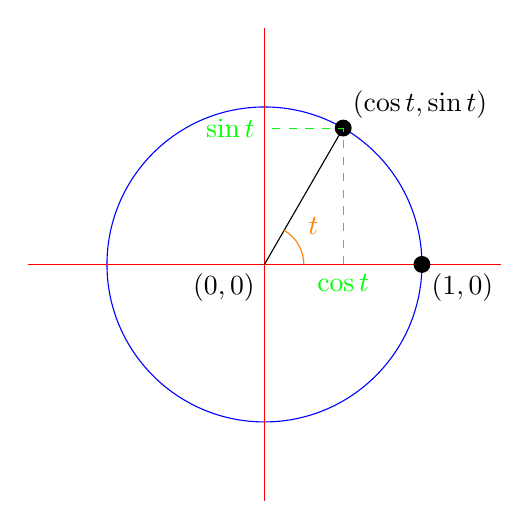
\begin{tikzpicture}
   \draw[color=blue] (0,0) circle (2);
   \draw[color=red] (-3,0) -- (3,0) (0,-3) -- (0,3);
   \draw (0,0) node[below left]{$(0,0)$} -- (1,1.732050807568877)
   circle (.1)[fill=black] node[above right]{$(\cos t,\sin t)$};
   \draw[color=green,dashed]
   (1,0) node[below]{$\cos t$} --
   (1,1.732050807568877) -- (0,1.732050807568877)
   node[left]{$\sin t$};
   \draw[color=orange] (.5,0) arc (0:30:.5) node[above right]{$t$}
   arc (30:60:.5);
   \draw (2,0) circle (.1)[fill=black] node[below right]{$(1,0)$};
 \end{tikzpicture}
\end{center}

\subsection{Ejercicio 3}

Plazar sobre el círculo unitario los puntos corespondiente a los 
  ángulos
    $-\frac{5\pi}{6}$,
    $-\frac{3\pi}{4}$,
    $-\frac{2\pi}{3}$,
    $-\frac{\pi}{2}$,
    $-\frac{\pi}{3}$,
    $-\frac{\pi}{4}$,
    $-\frac{\pi}{6}$,
    $0$,
    $\frac{\pi}{6}$,
    $\frac{\pi}{4}$,
    $\frac{\pi}{3}$,
    $\frac{\pi}{2}$,
    $\frac{2\pi}{3}$,
    $\frac{3\pi}{4}$,
    $\frac{5\pi}{6}$ y
    $\pi$.

\subsection{Ejercicio 4}

\begin{enumerate}
\item Sea $0 \leq t \leq \frac{\pi}{2}$. Place sobre el círculo unitario
  los puntos corespondientes a los ángulos $t, -t, t+\pi, \pi-t, t+2\pi$.
\item ¿Cómo se interpreta de manera gráfica el seno/coseno de $\alpha+2\pi$?
\item ¿Cómo se interpreta de manera gráfica el seno/coseno de $-\alpha$?
\item ¿Cómo se interpreta de manera gráfica el seno/coseno de $\pi-\alpha$?
\item ¿Cómo se interpreta de manera gráfica el seno/coseno de $\alpha+\pi$?
\item ¿Cómo se interpreta de manera gráfica la formula
  ${\left(\cos \left( x \right)\right)}^2 + {\left(\sin \left( x \right)\right)}^2 = 1$?
\end{enumerate}

\section{Soluciones de los ejercicios }

\subsection{Ejercicio 1}

\begin{enumerate}
\item coseno es decreciente y seno/tangente son creciente por la definición
  geométrica del capítulo VI (fijar la hipotenusa para coseno/seno y el lado
  adyacente para la tangente).
\item $\cos -x = \cos x$ significa que la gráfica del coseno es es simétrica
  con respecto al eje $y$. $\sin -x = -\sin x$ y $\tan -x = -\tan x$ significa
  que la gráfica del seno y tangente tiene una simétrica rotacional con
  respecto al origen de coordenada.
\item Eso (con la primera pregunta) indica que la gráfica del coseno es
  simétrica con respecto a todos los ejes vertícales
  $x = k \pi$ y que la gráfica del seno tiene una simétrica rotacional con
  respecto a todos los puntos$(k\pi, 0)$, donde $k \in \mathbb Z$.
\item $\sin\left(\alpha+\frac{\pi}{2}\right) = 
  \sin\left(-\left(\frac{\pi}{2}-\alpha\right) + \pi\right) =
  -\sin\left(-\left(\frac{\pi}{2}-\alpha\right)\right) =
  \sin\left(\frac{\pi}{2}-\alpha\right) = \cos \alpha$.  Entonces la gráfica
  del seno es la gráfica del coseno de desplazada de $\frac{\pi}{2}$ por la
  derecha.
\end{enumerate}

\subsection{Ejercicio 2}

\begin{enumerate}
\item ${BC} = 2\sin{\alpha}$ y $\overset{\frown}{BC} = 2\alpha$.
\item La cuerda $[BC]$ es más corte que el arco $\overset{\frown}{BC}$ y
  entonces $\sin{\alpha} \leq \alpha$. Por que $\sin -\alpha = -{\sin \alpha}$
  esta inegualidad se vuelve $\alpha \leq \sin{\alpha}$ cuando
  $-\frac{\pi}{2} \leq \alpha \leq 0$.
\item Para $x \in \left[-\frac{\pi}{2},\frac{\pi}{2}\right]$ trazamos la
  recta $y = x$ y la función $y = \sin x$. La gráfica del sino es
  abajo de esta recta si $x \geq 0$ y encima si $x \leq 0$. Utilizando las
  simetrías del seno y coseno, podemos generalizar este resultado.
\end{enumerate}

\subsection{Ejercicio 3}

\begin{center}
 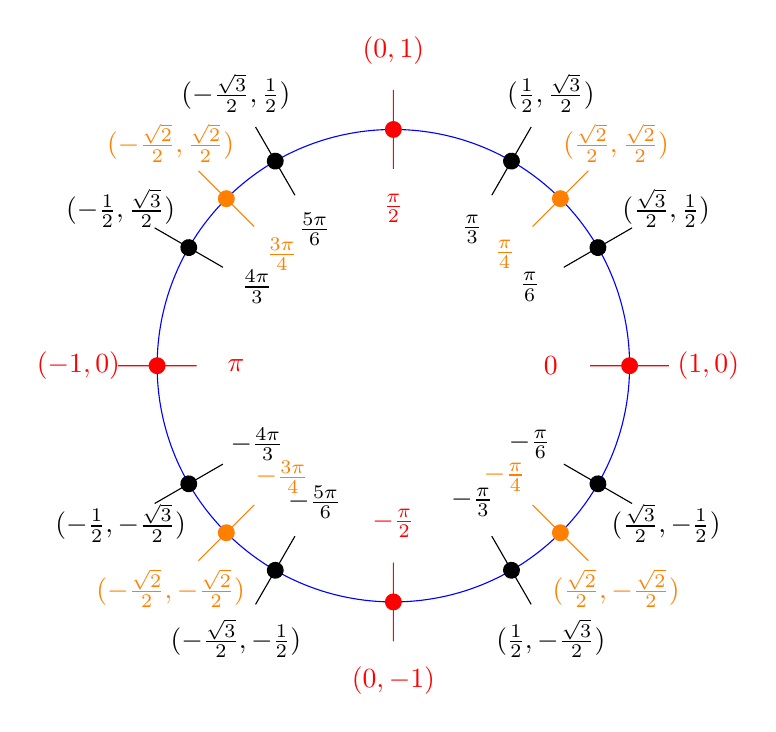
\begin{tikzpicture}
   \draw[color=blue] (0,0) circle (3);

   \begin{scope}[rotate around={0:(0,0)},color=red]
   \draw (2,0) node{$0$}
   (2.5,0) -- (3,0) circle (.1)[fill=red] -- (3.5,0)
   (4,0) node{$(1,0)$};
   \end{scope}

   \begin{scope}[rotate around={90:(0,0)},color=red]
   \draw (2,0) node{$\frac{\pi}{2}$}
   (2.5,0) -- (3,0) circle (.1)[fill=red] -- (3.5,0)
   (4,0) node{$(0,1)$};
   \end{scope}

   \begin{scope}[rotate around={180:(0,0)},color=red]
   \draw (2,0) node{$\pi$}
   (2.5,0) -- (3,0) circle (.1)[fill=red] -- (3.5,0)
   (4,0) node{$(-1,0)$};
   \end{scope}

   \begin{scope}[rotate around={-90:(0,0)},color=red]
   \draw (2,0) node{$-\frac{\pi}{2}$}
   (2.5,0) -- (3,0) circle (.1)[fill=red] -- (3.5,0)
   (4,0) node{$(0,-1)$};
   \end{scope}
   %%%%%%%%%%
   \begin{scope}[rotate around={30:(0,0)}]
   \draw (2,0) node{$\frac{\pi}{6}$}
   (2.5,0) -- (3,0) circle (.1)[fill=black] -- (3.5,0)
   (4,0) node{$(\frac{\sqrt{3}}{2},\frac{1}{2})$};
   \end{scope}

   \begin{scope}[rotate around={45:(0,0)},color=orange]
   \draw (2,0) node{$\frac{\pi}{4}$}
   (2.5,0) -- (3,0) circle (.1)[fill=orange] -- (3.5,0)
   (4,0) node{$(\frac{\sqrt{2}}{2},\frac{\sqrt{2}}{2})$};
   \end{scope}

   \begin{scope}[rotate around={60:(0,0)}]
   \draw (2,0) node{$\frac{\pi}{3}$}
   (2.5,0) -- (3,0) circle (.1)[fill=black] -- (3.5,0)
   (4,0) node{$(\frac{1}{2},\frac{\sqrt{3}}{2})$};
   \end{scope}
   %%%%%%%%%%
   \begin{scope}[rotate around={120:(0,0)}]
   \draw (2,0) node{$\frac{5\pi}{6}$}
   (2.5,0) -- (3,0) circle (.1)[fill=black] -- (3.5,0)
   (4,0) node{$(-\frac{\sqrt{3}}{2},\frac{1}{2})$};
   \end{scope}

   \begin{scope}[rotate around={135:(0,0)},color=orange]
   \draw (2,0) node{$\frac{3\pi}{4}$}
   (2.5,0) -- (3,0) circle (.1)[fill=orange] -- (3.5,0)
   (4,0) node{$(-\frac{\sqrt{2}}{2},\frac{\sqrt{2}}{2})$};
   \end{scope}

   \begin{scope}[rotate around={150:(0,0)}]
   \draw (2,0) node{$\frac{4\pi}{3}$}
   (2.5,0) -- (3,0) circle (.1)[fill=black] -- (3.5,0)
   (4,0) node{$(-\frac{1}{2},\frac{\sqrt{3}}{2})$};
   \end{scope}
   %%%%%%%%%%
   \begin{scope}[rotate around={-30:(0,0)}]
   \draw (2,0) node{$-\frac{\pi}{6}$}
   (2.5,0) -- (3,0) circle (.1)[fill=black] -- (3.5,0)
   (4,0) node{$(\frac{\sqrt{3}}{2},-\frac{1}{2})$};
   \end{scope}

   \begin{scope}[rotate around={-45:(0,0)},color=orange]
   \draw (2,0) node{$-\frac{\pi}{4}$}
   (2.5,0) -- (3,0) circle (.1)[fill=orange] -- (3.5,0)
   (4,0) node{$(\frac{\sqrt{2}}{2},-\frac{\sqrt{2}}{2})$};
   \end{scope}

   \begin{scope}[rotate around={-60:(0,0)}]
   \draw (2,0) node{$-\frac{\pi}{3}$}
   (2.5,0) -- (3,0) circle (.1)[fill=black] -- (3.5,0)
   (4,0) node{$(\frac{1}{2},-\frac{\sqrt{3}}{2})$};
   \end{scope}
   %%%%%%%%%%
   \begin{scope}[rotate around={-120:(0,0)}]
   \draw (2,0) node{$-\frac{5\pi}{6}$}
   (2.5,0) -- (3,0) circle (.1)[fill=black] -- (3.5,0)
   (4,0) node{$(-\frac{\sqrt{3}}{2},-\frac{1}{2})$};
   \end{scope}

   \begin{scope}[rotate around={-135:(0,0)},color=orange]
   \draw (2,0) node{$-\frac{3\pi}{4}$}
   (2.5,0) -- (3,0) circle (.1)[fill=orange] -- (3.5,0)
   (4,0) node{$(-\frac{\sqrt{2}}{2},-\frac{\sqrt{2}}{2})$};
   \end{scope}

   \begin{scope}[rotate around={-150:(0,0)}]
   \draw (2,0) node{$-\frac{4\pi}{3}$}
   (2.5,0) -- (3,0) circle (.1)[fill=black] -- (3.5,0)
   (4,0) node{$(-\frac{1}{2},-\frac{\sqrt{3}}{2})$};
   \end{scope}
 \end{tikzpicture}
\end{center}

\subsection{Ejercicio 4}


\begin{enumerate}

\item

\begin{center}
 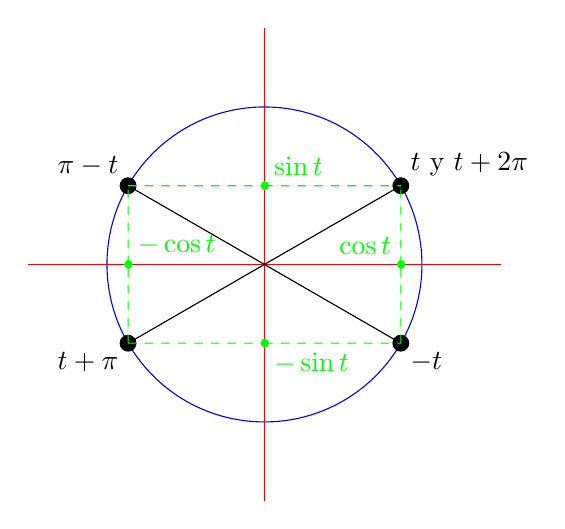
\begin{tikzpicture}
   \draw[color=blue] (0,0) circle (2);
   \draw[color=red] (-3,0) -- (3,0) (0,-3) -- (0,3);
   \draw (0,0) -- (1.732050807568877,1)
   circle (.1)[fill=black] node[above right]{$t$ y $t+2\pi$};
   \draw (0,0) -- (-1.732050807568877,1)
   circle (.1)[fill=black] node[above left]{$\pi-t$};
   \draw (0,0) -- (1.732050807568877,-1)
   circle (.1)[fill=black] node[below right]{$-t$};
   \draw (0,0) -- (-1.732050807568877,-1)
   circle (.1)[fill=black] node[below left]{$t+\pi$};

   \draw[color=green,dashed]
   (-1.732050807568877,1) --
   (0,1) circle(.05)[fill=green] node[above right]{$\sin t$} --
   (1.732050807568877,1);

   \draw[color=green,dashed]
   (-1.732050807568877,-1) --
   (0,-1) circle(.05)[fill=green] node[below right]{$-\sin t$} --
   (1.732050807568877,-1);

   \draw[color=green,dashed]
   (1.732050807568877,-1) --
   (1.732050807568877,0) circle(.05)[fill=green]
   node[above left]{$\cos t$} --
   (1.732050807568877,1);

   \draw[color=green,dashed]
   (-1.732050807568877,-1) --
   (-1.732050807568877,0) circle(.05)[fill=green]
   node[above right]{$-\cos t$} --
   (-1.732050807568877,1);

 \end{tikzpicture}
\end{center}

\item Hacer una vuelta no cambía su posición sobre el círculo unitario.
  Entonces $\cos {(t+2\pi)} = \cos t$ y $\sin {(t+2\pi)} = \sin t$.

\item Si andamos la misma distancia en sentidos opuestos
  obtenemos dos puntos símetricos con respecto al eje $x$.
  Entonces $\cos -t = \cos t$ y $\sin -t = -\sin t$.
\item Si andamos una distancia desde el punto $(1,0)$
  y la misma distancia en sentido opuesto desde el punto $(-1,0)$,
  obtemeos puntos símetricos con respecto al eje $y$.
  Entonces $\cos {(\pi-t)} = -\cos t$ y $\sin {(\pi-t)} = \sin t$.

\item Si andamos una distancia desde el punto $(1,0)$
  y la misma distancia desde el punto $(-1,0)$, obtemeos puntos símetricos con
  respecto al punto $(0,0)$.
  Entonces $\cos {(\pi+t)} = -\cos t$ y $\sin {(\pi+t)} = -\sin t$.

\item Todos los puntos $(\cos t, \sin t)$
  del círculo unitario están a una distancia $1$ del
  centro $(0,0)$ entonces
  $1= \sqrt{{\left(\cos \left( x \right) - 0\right)}^2 + {\left(\sin \left( x \right) - 0\right)}^2}$.
\end{enumerate}
